\documentclass[a4paper, 12pt]{article}
\usepackage[a4paper,top=1.5cm, bottom=1.5cm, left=1cm, right=1cm]{geometry}
\usepackage{cmap}					
\usepackage{mathtext} 				
\usepackage[T2A]{fontenc}			
\usepackage[utf8]{inputenc}			
\usepackage[english,russian]{babel}
\usepackage{multirow}
\usepackage{graphicx}
\usepackage{wrapfig}
\usepackage{tabularx}
\usepackage{float}
\usepackage{longtable}
\usepackage{hyperref}
\hypersetup{colorlinks=true,urlcolor=blue}
\usepackage[rgb]{xcolor}
\usepackage{amsmath,amsfonts,amssymb,amsthm,mathtools} 
\usepackage{icomma} 
\usepackage{euscript}
\usepackage{mathrsfs}
\usepackage{enumerate}
\usepackage{caption}
\usepackage{enumerate}
\mathtoolsset{showonlyrefs=true}
\usepackage{graphicx}
\usepackage{caption}
\usepackage{subcaption}
\usepackage[europeanresistors, americaninductors]{circuitikz}
\DeclareMathOperator{\sgn}{\mathop{sgn}}
\newcommand*{\hm}[1]{#1\nobreak\discretionary{}
	{\hbox{$\mathsurround=0pt #1$}}{}}

\title{\textbf{Изучение колебаний струны (1.4.5)}}
\author{Манро Эйден}
\date{}

\begin{document}

\maketitle
	      	
    \begin{center}
    \section*{Введение}    
    \end{center}


    \noindent \textbf{Цель работы:} исследовать зависимости частоты колебаний струны от величины натяжения, а также условий установления стоячей волны, получающейся в результате сложения волн, идущих в противоположных направлениях.

    \bigskip

    \noindent \textbf{Оборудование:} звуковой генератор, двухканальный осциллограф, постоянный магнит, набор грузов, рейка со струной.

    \bigskip
    
    \begin{center}
         \subsection*{Теоретические сведения}
    \end{center}
    
    \par Основное свойство струны -- гибкость, является следствием ее большой длины по сравнению с поперечными размерами. Даже струны, изготовленные из жестких материалов, практически не сопротивляются изгибанию, если размер изгибаемого участка значительно больше поперечного размера струны. Данный факт позволяет не учитывать при дальнейшей работе изгибные напряжения.
	
	Горизонтально закрепленная струна провисает под действием поля тяжести, при отсутствии натяжения. Достаточно натянутую струну можно считать прямой, если ее концы закреплены на одном горизонтальном уровне. Учитывая этот факт, в дальнейшем действие силы тяжести учитываться не будет.
	
	Натянутая струна с жестко закрепленными концами удобна для изучения колебаний. Это связанно с тем, что в струне можно непосредственно наблюдать простейшие типы колебаний и волн, измерять их параметры и сравнивать результаты наблюдения с результатами теоретических расчетов.
	
	Движение элементов струны может быть вызвано изменением ее формы или передачей ей импульса. Натяжение струны стремиться вернуть ее в изначальное прямолинейное положение, и это приводит к тому, что возникает движение элементов струны. Возмущения бегут вдоль струны.
	
	Скорость распространения подобного возмущения можно вычислить по формуле:

    \begin{center}

        \begin{equation}
		u = \sqrt{\frac{T}{\rho_l}},
            \label{velocity_of_deformation}
	\end{equation}
    где $T$ -- сила натяжения струны, $\rho_{l}$ -- масса струны на единицу длины.

    \begin{equation}
		\lambda = \frac{u}{\nu}
	\end{equation}
	
	Частоты собственных колебаний струны определяются формулой:
	
	\begin{equation}
		\nu_{n} = \frac{nu}{2l} = \frac{n}{2l}\sqrt{\frac{T}{\rho_l}}
            \label{frequency_velocity_equation}
	\end{equation}
	где $n$ -- число полуволн, $l$ -- длина струны.
    \end{center}

    \newpage
    
    \begin{center}
        \subsection*{Экспериментальная установка}

        \begin{figure}[h!]
		\begin{center}
			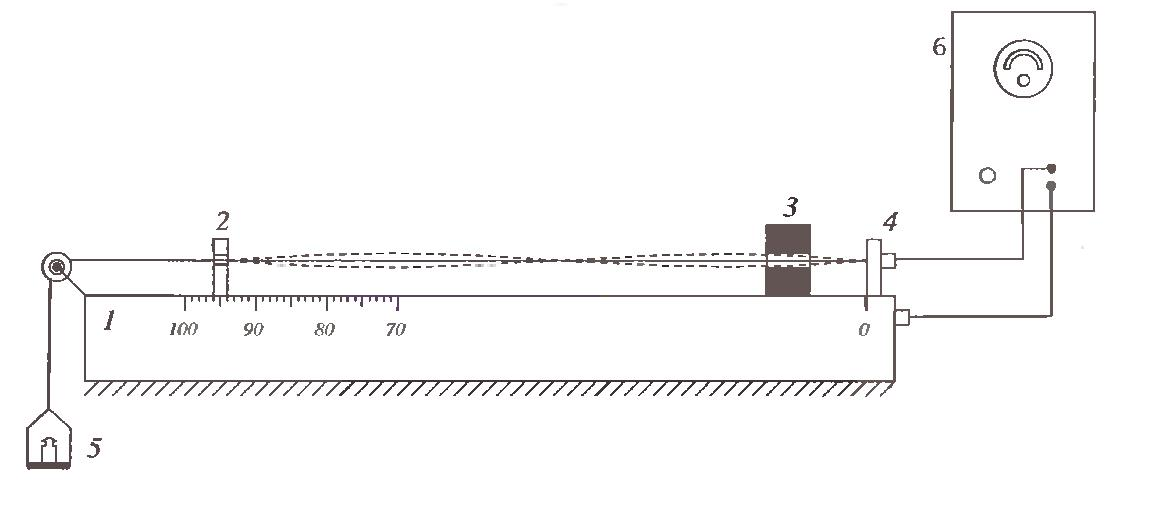
\includegraphics[width = 0.9\textwidth]{exp145.jpg}
			\caption{Схема экспериментальной установки}
		\end{center}
	\end{figure}
 
    \end{center}

        На Рисунке 1 представлена схема экспериментальной установки. Устроена она следующим образом: на массивной металлической рейке 1 установлены опора 2 и магнит 3, которые можно перемещать вдоль рейки, а также неподвижная опора 4. Один конец струны закреплен в изоляторе опоры 4. От него струна проходит между полюсами магнита и через опору 2, которая дает возможность струне перемещаться в горизонтальной плоскости, неподвижный блок и соединяется с чашкой 5, на которую помещаются грузы. Такое устройство позволяет регулировать натяжение струны. К концу струны, закрепленному в изоляторе опоры 4, и к массивной металлической рейке 1 подводится переменное напряжение от звукового генератора 6. Движение струны вызывается силой Ампера, действующей на проводник с током со стороны магнитного поля. Частота колебания струны совпадает с частотой вынуждающей силы, т.е с частотой силы Ампера. Так как данная сила зависит от тока в проводнике, то частота колебаний струны будет совпадать с частотой генератора.
	
	В натянутой струне возникнут колебания и по ней побегут волны, которые отразятся от опор 2 и 4 и, сложившись друг с другом, создадут стоячую волну, если на длине струны уложится целое число полуволн.

    \begin{center}
        \section*{Ход работы}
        $T = (m_\text{пл} + \sum\limits_{i=1}^n m_i)g,$ 
        где $m_\text{пл} = 118$ гр - масса платформы, $m_i$ - масса груза.
        
        \bigskip
        
        Подставляя значения в формулу \eqref{frequency_velocity_equation} получаем значения частот основной гармоники для разных масс:
    \end{center}

    \begin{table}[!h]
        \begin{center}
		\begin{tabular}{|c|c|c|c|c|}
			\hline
			$\nu_1$, Гц &$\nu_2$, Гц& $\nu_3$, Гц& $\nu_4$, Гц& $\nu_5$, Гц\\
			\hline
			137 & 165 & 189 & 210 & 229\\
			\hline 
		\end{tabular}
  
	    \caption{Частоты основной гармоники}
        \end{center}
    \end{table}

    \newpage

     \begin{table}[!h]
        \begin{center}
		\begin{tabular}{|c|c|c|c|c|}
			\hline
			$M_1$, гр & $M_2$, гр & $M_3$, гр & $M_4$, гр & $M_5$, гр\\
			\hline
			  1096 & 1588 & 2081 & 2568 & 3056\\
			\hline 
		\end{tabular}
  
	    \caption{Суммарная масса}
        \end{center}
    \end{table}
    \begin{center}
        С помощью осциллографа будем находить частоты гармоник с 1 до 10. 
    \end{center}
	\begin{table}[!h]
		\begin{center}
			\begin{tabular}{|c|c|c|c|c|c|c|c|c|c|c|c|}
				\hline
				$T$, Н& $\nu_1$, Гц &$\nu_2$, Гц& $\nu_3$, Гц& $\nu_4$, Гц& $\nu_5$, Гц& $\nu_6$, Гц &$\nu_7$, Гц& $\nu_8$, Гц& $\nu_9$, Гц& $\nu_{10}$, Гц\\
				\hline
				11 & 138 & 276 & 415 & 554 & 695 & 838 & 977 & 1122 & 1259 & 1399\\ 
				\hline
				16 & 164 & 328 & 494 & 658 & 825 & 991 & 1158 & 1324 & 1494 & 1663\\ 
				\hline
				20 & 190 & 380 & 572 & 763 & 954 & 1146 & 1338 & 1531 & 1724 & 1920\\
				\hline
				25 & 211 & 421 & 631 & 842 & 1053 & 1263 & 1476 & 1686 & 1902 & 2116\\ 
				\hline
				30 & 230 & 461 & 691 & 922 & 1154 & 1385 & 1617 & 1850 & 2083 & 2317\\ 
				\hline
			\end{tabular}
		\caption{Снятые результаты частот гармоник}
		\end{center}
	\end{table}
    \begin{center}
        Построим график зависимости $\nu_n$ от $n$ по МНК:
    \end{center}
    
    \begin{figure}[h!]
        \begin{center}
            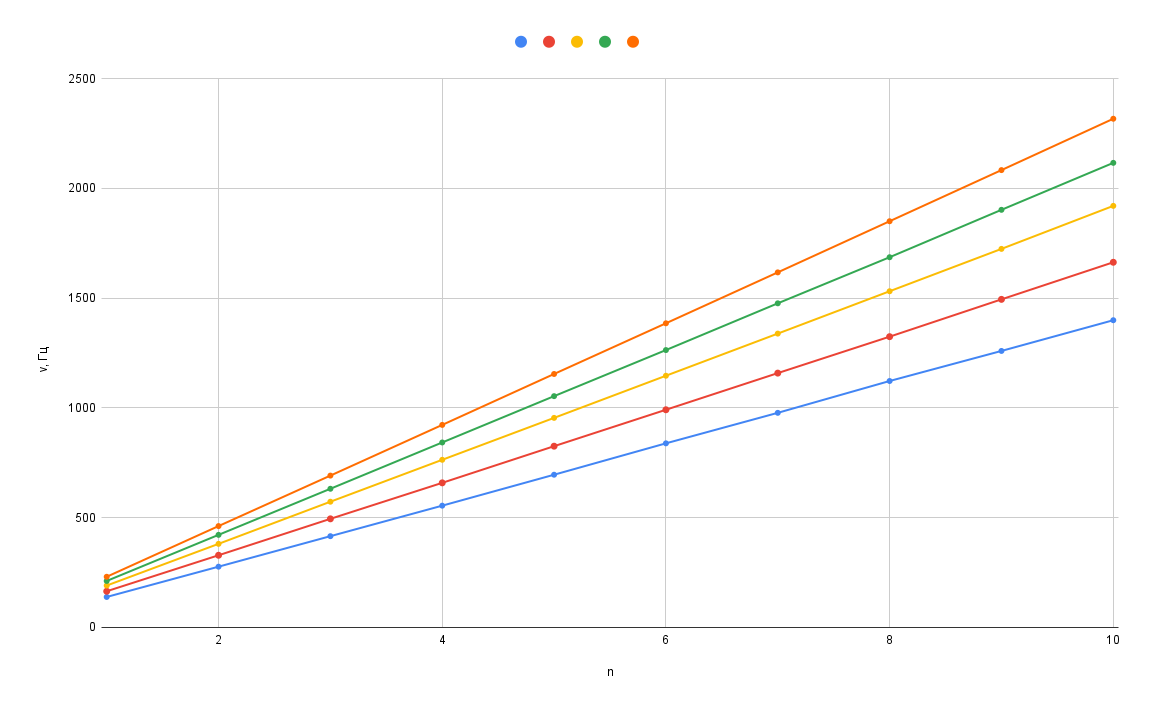
\includegraphics[width = 1.0\textwidth]{chart.png}
            \caption{График зависимости $\nu_n (n)$}
        \end{center}
    \end{figure}

    \newpage
    
    \begin{center}
    
    Воспользуемся формулой \eqref{frequency_velocity_equation}, получаем, что угол наклона графика $k = \dfrac{u}{2l}$. Еще воспользуемся МНК-аппроксимацией и получим погрешности для $u$:

    \end{center}

    \begin{itemize}
        \begin{center}
		\item $T = 11$, Н -- $u = (139,7 \pm 1,2)$, м/с
		\item  $T = 16$, Н -- $u = (165,7 \pm 1,4)$, м/с
		\item  $T = 20$, Н -- $u = (191,4 \pm 1,1)$, м/с
		\item  $T = 25$, Н -- $u = (211,1 \pm 1,1)$, м/с
		\item  $T = 30$, Н -- $u = (231,2 \pm 1,0)$, м/с
        \end{center}
    \end{itemize}

    \begin{center}
        
    С помощью полученных данных построим график зависимости $u^2(T)$, для того, чтобы найти линейную плотность струны $ \rho_l $. 
	
	\begin{figure}[h!]
		\begin{center}
			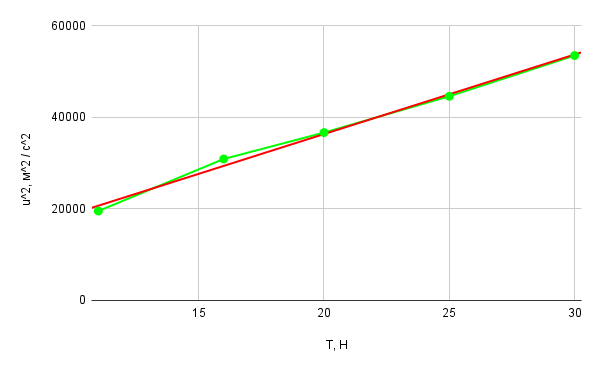
\includegraphics[scale=0.8]{chart1.png}
			\caption{Зависимость $ u^2 $ от $ T $}
			\label{chart1}
		\end{center}
	\end{figure}

    \end{center}

    \begin{center}
        
    С помощью формулы \eqref{velocity_of_deformation}, можно понять, что коэффицент наклона $k$, для графика \ref{chart1}, будет равен: $$k = \dfrac{1}{\rho_l}$$ Аналогично воспользуемся МНК-аппроксимацией и получим погрешности для $k$ и соответственно для $\rho_l$.

    \bigskip
    
    Таким образом $k = (1737 \pm 77) {, \dfrac{\text{м}}{\text{кг}}} $.
	Тогда $\rho_l = (575,7 \pm 12,9) \text{, $\dfrac{\text{мг}}{\text{м}}$}$.
    \end{center}

    \newpage

    \begin{center}
        Полученное значение соответствует истинному значению погонной плостности струны, которая равняется $\rho^{\text{ист}}_l = 568,4\text{, $\dfrac{\text{мг}}{\text{м}}$} $.
    \end{center}

\begin{center}

    \section*{Вывод}
В работе были изучены поперечные стоячие волны на тонкой натянутой струне, были измерены собственные частоты её колебаний, измерена скорость распространения волн в струне и линейная плотность струны. Экспериментальные графики зависимостей $\nu_n(n)$ и $u^2(T)$ хорошо ложатся на аппроксимирующие прямые. Отклонение аппроксимирующих прямых от начала координат по оси ординат мало ($\sim 1\%$) по сравнению с значениями ординат экспериментальных точек. Отличие измеренного значения линейной плотности струны от указанного на установке составляет $2 \%$.
Погрешности связаны с
\begin{itemize}
\item[1) ] Неточностью определения собственных частот $\nu_n$ из-за возникновения нелинейных эффектов при резонансе, и, как следствие, неточностью в определении скорости распространения $u$ волны в струне.
\item[2) ] Недостаточным количеством экспериментальных точек на графике $u^2(T)$, то есть недостаточным количеством опытов по измерению собственных частот струны в зависимости от силы натяжения нити $T$.
\end{itemize}
\end{center}
 

    
    

    
    
   
\end{document}
